\section{The Perceptron Algorithm and its Variants}\label{sec:q3}

\begin{enumerate}

	\item
		\begin{enumerate}
	
			\item Python3.6 is used to implement the experiment.\\
			\item Each datafile is read and parsed into a numpy array with 68 columns. Each column has appropriate values of the features as in the file. Rest are set to 0.\\
			\item I have defined perceptron as a single class with training data, test data, predictions, weights, bias and accuracy as its attributes and train and predict as its methods. The file $perceptron.py$ represents the class. Aggressive variants of train and predict methods are also present in the class and called when aggressive flag is set while calling train and predict. Weights are represented by a list of floats with length equal to that of number of columns. Bias is represented as float. When object of perceptron class is created, the weights and bias are initialised randomly between $-0.01$ and $0.01$. There is option of seeding this random number if required.\\
			
			\item Simple perceptron is represented by the class as is. No extra parameters except for data and learning rate are required while calling the train function.\\
				If dynamic\_ lr flag for train function is set, then perceptron will learn with a dynamic learning rate. The learning rate is updated for each example, whether there is a mistake or not.\\
				While creating object of perceptron object we can pass it margin value which is used to check if update is to be done for the example or not. Default value of this attribute is $0$.\\
				There are extra attributes to store average weights and average bias. These are always updated in each iteration, but the predict function ignores them unless average flag is set, in this case average weights and average bias are used for prediction.\\ 
				Aggressive perceptron can be trained by passing the aggressive flag as 1 in train and predict function. Here weights and bias are not stored seperately but collection of weights has $n+1$ weights where $n$ is number of features in data. An column of $1$s is appended to $x$ before training and predictions.
				
			\item
			I have used a two random functions. One for generation of random weights and bias, and the other for shuffling numpy arrays. Both can be seeded to have output as described in trace file.
			Seed value can be set by setting the variable in $random\_seed.py$ file. Just uncomment the lines which are used to set the random seed, in order to seed those functions
			
		\end{enumerate}	
	
	\item
	The number of instances of each label in training set:
	$$1 	= 4606 $$
	$$-1 = 3685 $$
	
	The number of instances of each label in dev set:
	$$1 	= 759 $$
	$$-1 = 623 $$
	
	The number of instances of each label in test set:
	$$1 	= 792 $$
	$$-1 = 590 $$
	
	Let us consider a classifier which predicts the most frequent label. So this classifer will train will always predict the majority label $1$.
	
	Accuracy on dev set: \\
	$A_{dev} = 759/(759+623)*100 = 54.92 \%$
	
	Accuracy on test set: \\
	$A_{test} = 792/(792+590)*100 = 57.30 \%$
	
	\item
	The following results are for when seed in $random\_seed.py$ file is set to 6.111
	\begin{enumerate}
		\item Simple Perceptron
			\begin{enumerate}
				\item Best Hyperparameter: learning rate = 0.1
				\item Cross Validation accuracy for best hyperparameter: 90.7971
				\item Total number of updates performed on training set: 14086
				\item Development set accuracy: 90.6657
				\item Test set accuracy: 92.9088
				\item Epoch vs Dev Set Accuracy:
					\begin{center}
						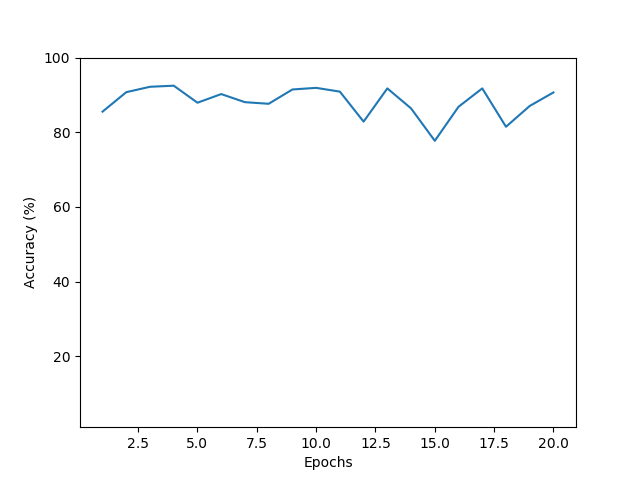
\includegraphics[scale=0.7]{Simple}
					\end{center}
			\end{enumerate}
			
		\item Perceptron with dynamic learning rate
			\begin{enumerate}
				\item Best Hyperparameter: Initial Learning Rate = 1
				\item Cross Validation accuracy for best hyperparameter: 89.2898
				\item Total number of updates performed on training set: 16408
				\item Development set accuracy: 90.8104
				\item Test set accuracy: 91.3893
				\item Epoch vs Dev Set Accuracy:
					\begin{center}
						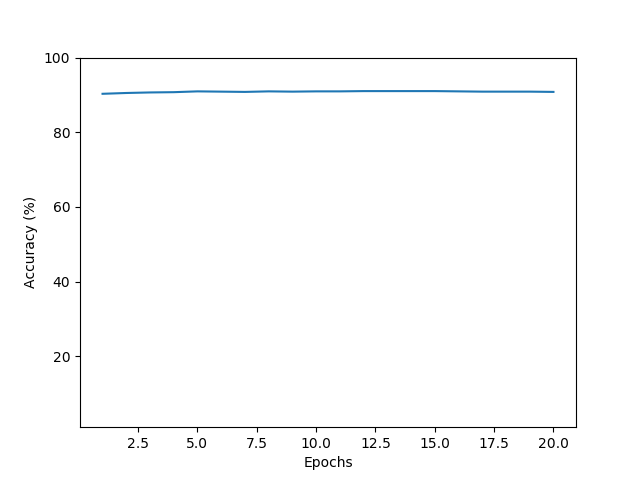
\includegraphics[scale=0.7]{Dynamic}
					\end{center}
			\end{enumerate}

		\item Perceptron with margin
			\begin{enumerate}
				\item Best Hyperparameter:\\ Intial learning rate = 1\\ Margin = 0.1
				\item Cross Validation accuracy for best hyperparameter: 91.0869
				\item Total number of updates performed on training set: 73105
				\item Development set accuracy: 90.521
				\item Test set accuracy: 92.2576
				\item Epoch vs Dev Set Accuracy:
					\begin{center}
						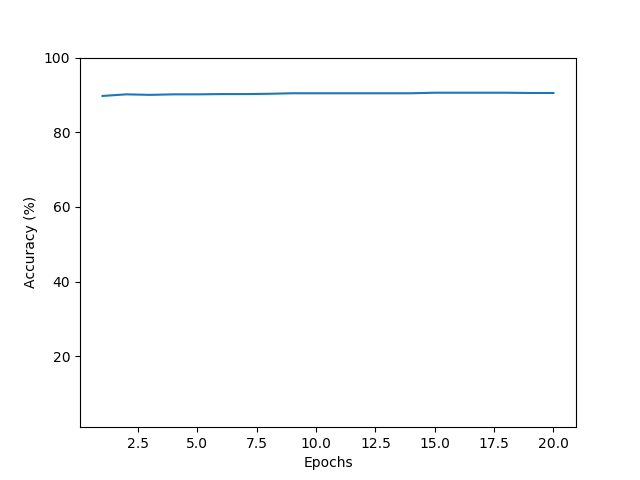
\includegraphics[scale=0.7]{Margin}
					\end{center}
			\end{enumerate}
			
		\item Averaged Perceptron
			\begin{enumerate}
				\item Best Hyperparameter: Learning Rate = 0.01
				\item Cross Validation accuracy for best hyperparameter: 93.5835
				\item Total number of updates performed on training set: 14027
				\item Development set accuracy: 92.4023
				\item Test set accuracy: 92.9812
				\item Epoch vs Dev Set Accuracy:
					\begin{center}
						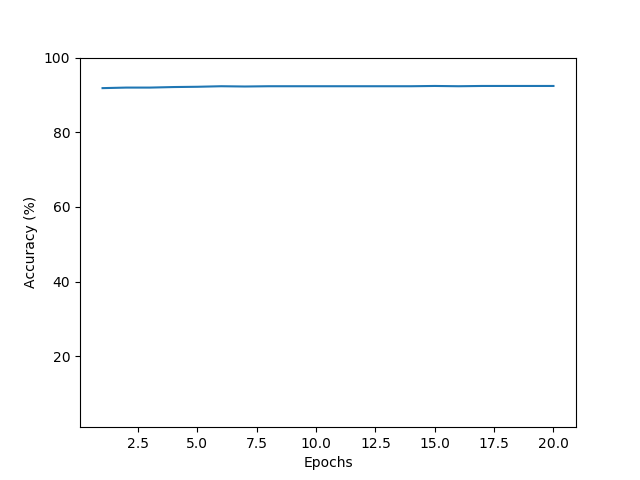
\includegraphics[scale=0.7]{Averaged}
					\end{center}
			\end{enumerate}

		\item Aggressive Perceptron with margin
			\begin{enumerate}
				\item Best Hyperparameter: Margin = 0.1
				\item Cross Validation accuracy for best hyperparameter: 88.2397
				\item Total number of updates performed on training set: 63574
				\item Development set accuracy: 91.8234
				\item Test set accuracy: 93.1983
				\item Epoch vs Dev Set Accuracy:
					\begin{center}
						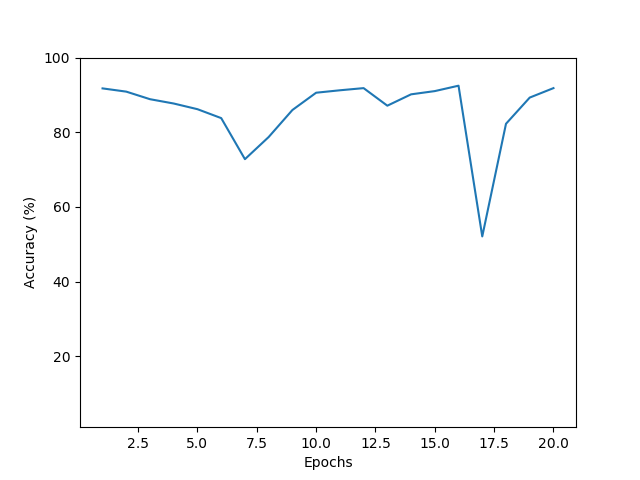
\includegraphics[scale=0.7]{aggressive}
					\end{center}
			\end{enumerate}	
	
	\end{enumerate}

\end{enumerate}